\chapter{بازنمایی متن در \eng{TTS}: از \eng{One-Hot} تا بازنمایی وابسته به بافت}

\section{مروری بر معماری سامانه‌های تبدیل متن به گفتار}

سامانه‌های \term{تبدیل متن به گفتار}{Text-to-Speech} را می‌توان به دو شکل ساخت: \term{معماری خط‌لوله‌ای}{Pipeline-Based} (چند ماژول مستقل که خروجی هر یک ورودی بعدی است) و \term{معماری سرتاسری}{End-to-End} (یک مدل یکپارچه). تمرکز فعلی درس بر معماری خط‌لوله‌ای است تا هر ماژول را جداگانه بشناسیم.

\begin{figure}[htbp]
\centering
\begin{tikzpicture}[rtl,
  node distance=4mm,
  box/.style={draw, rounded corners=2pt, minimum height=9mm, minimum width=24mm, align=center, font=\small},
  front/.style={box, fill=blue!10},
  back/.style={box, fill=orange!15},
  arr/.style={-{Stealth[length=2.2mm]}, thick}
]
\node[box, fill=gray!10] (txt) {\RL{متن ورودی}\\\lr{Input Text}};
\node[front, below=of txt] (norm) {\RL{نرمال‌سازی متن}\\\lr{Text Normalization}};
\node[front, below=of norm] (homo) {\RL{رفع ابهام هم‌نویسه‌ها}\\\lr{Homograph Disambiguation}};
\node[front, below=of homo] (g2p) {\RL{تولید توالی واج}\\\lr{Phoneme Generation}};
\node[back, right=14mm of g2p] (spec) {\RL{تولید طیف‌نگاشت}\\\lr{Spectrogram Generation}};
\node[back, above=of spec] (wav) {\RL{تولید موج صوتی}\\\lr{Speech Waveform}};
\draw[arr] (txt)--(norm); \draw[arr] (norm)--(homo); \draw[arr] (homo)--(g2p);
\draw[arr] (g2p)--(spec); \draw[arr] (spec)--(wav);
\node[font=\small\bfseries, blue!60!black, left=4mm of homo] {\lr{Front-End}};
\node[font=\small\bfseries, orange!60!black, above=2mm of wav] {\lr{Back-End}};
\end{tikzpicture}
\caption{مراحل معماری خط‌لوله‌ای \eng{TTS}: سه مرحلهٔ آبی «بخش پیشین» و دو مرحلهٔ نارنجی «بخش پسین» است.}
\end{figure}

\begin{definitionbox}{بخش پیشین و بخش پسین}
\term{بخش پیشین}{Front-End} با \emph{متن} کار می‌کند (نرمال‌سازی، رفع ابهام، استخراج اطلاعات تلفظی). \term{بخش پسین}{Back-End} با بازنمایی‌های \emph{صوتی} سروکار دارد و صدای نهایی را می‌سازد. این دو با مفاهیم هم‌نام در توسعهٔ وب ارتباطی ندارند.
\end{definitionbox}

\begin{exambox}{تأکید استاد دربارهٔ ماژولار بودن}
هر ماژول را باید جداگانه یاد گرفت؛ زیرا ممکن است در پروژه‌ای به یکی از آن‌ها بیشتر نیاز داشته باشیم یا بخواهیم چند ماژول را ادغام کنیم. مدل‌های بزرگ سرتاسری از نظر منابع محاسباتی و \term{تأخیر}{Latency} محدودیت دارند؛ پس شناخت معماری‌های کوچک و ماژولار همچنان مهم است.
\end{exambox}

\textbf{هدف اصلی این جلسه:} تشخیص تلفظ درست \term{هم‌نویسه‌ها}{Homograph} با استفاده از بازنمایی کلمات و بافت جمله. برای این کار باید بدانیم کلمه چگونه به شبکهٔ عصبی داده می‌شود و شبکه چگونه آموزش می‌بیند.

\section{بازنمایی متن برای شبکه‌های عصبی}

شبکه‌های عصبی مستقیماً با کلمات کار نمی‌کنند و به بازنمایی عددی نیاز دارند.

\subsection{بازنمایی \eng{One-Hot}}
در بردار \term{تک‌داغ}{One-Hot} برای واژگانی با $V$ کلمه، هر کلمه برداری به طول $V$ است که فقط مؤلفهٔ متناظر با اندیس کلمه ۱ و بقیه صفرند (مثلاً کلمهٔ سوم از پنج کلمه: $(0,0,1,0,0)$). چهار محدودیت مهم:
\begin{enumerate}
  \item \textbf{ابعاد زیاد:} طول بردار برابر اندازهٔ واژگان است.
  \item \textbf{پراکنده بودن (\eng{Sparse}):} بیشتر مؤلفه‌ها صفرند.
  \item \textbf{تعامد (\eng{Orthogonality}):} ضرب داخلی هر دو بردار متفاوت صفر است.
  \item \textbf{نبود شباهت معنایی:} کلمات هم‌معنا یا هم‌گروه (مثلاً نام دو شهر) هیچ نزدیکی عددی ندارند.
\end{enumerate}
ریشهٔ مشکل: کلمات بر اساس \term{بافت}{Context} و \term{هم‌وقوعی}{Co-occurrence} به هم مرتبط‌اند و \eng{One-Hot} هیچ‌یک را نشان نمی‌دهد.

\subsection{بازنمایی توزیع‌شده: \eng{Word Embedding}}
در \term{تعبیهٔ کلمه}{Word Embedding} یک بُعد دلخواه (مثلاً ۱۲۸ یا ۳۰۰) انتخاب و به هر کلمه برداری با همین طول نسبت داده می‌شود. هر مؤلفه یک ویژگی عددی است که در آموزش یاد گرفته می‌شود و لازم نیست از ابتدا معنایش مشخص باشد.

\coursefigure{0.32}{ch08-onehot-vs-dense.png}{مقایسهٔ بردارهای \eng{One-Hot} (پراکنده، با ابعاد زیاد و ازپیش‌تعریف‌شده) و \eng{Embedding} (متراکم، با ابعاد کم‌تر و آموخته‌شده از داده).}

\begin{table}[htbp]
\centering
\caption{مقایسهٔ دو بازنمایی}
\begin{tabular}{l c c}
\toprule
ویژگی & \eng{One-Hot} & \eng{Embedding} \\
\midrule
تراکم & پراکنده (\eng{Sparse}) & متراکم (\eng{Dense}) \\
بُعد & برابر اندازهٔ واژگان & کوچک و دلخواه \\
چگونگی ساخت & ازپیش‌تعریف‌شده & آموخته از داده \\
شباهت معنایی & ندارد & دارد \\
\bottomrule
\end{tabular}
\end{table}

\begin{definitionbox}{بازنمایی توزیع‌شده در برابر پراکنده}
در بازنمایی پراکنده هر کلمه یک خانهٔ روشن منحصربه‌فرد است. در بازنمایی \term{توزیع‌شده}{Distributed} معنای هر کلمه در چند مؤلفه پخش می‌شود و هر مؤلفه در بازنمایی چندین کلمه نقش دارد؛ به همین دلیل فاصله و زاویهٔ میان بردارها معنا پیدا می‌کند.
\end{definitionbox}

\subsection{بردارهای \eng{Embedding} چگونه یاد گرفته می‌شوند؟}
بردارها ابتدا تصادفی مقداردهی می‌شوند و سپس یک \term{وظیفهٔ آموزشی}{Task} تعریف می‌شود. چرخهٔ یادگیری: دریافت ورودی، پیش‌بینی خروجی، مقایسه با مقدار صحیح (\eng{Ground Truth})، محاسبهٔ خطا و تغییر وزن‌ها برای کاهش خطا. بردارهای \eng{Embedding} نیز پارامتر قابل یادگیری‌اند و پس از آموزش می‌توان فقط آن‌ها را برداشت و در مدل‌های دیگر به کار برد.

یک وظیفهٔ رایج، پنهان‌کردن بخشی از جمله است: «من امروز به \eng{[MASK]} رفتم.» مدل باید از کلمات اطراف حدس بزند. مزیت: به برچسب‌گذاری دستی نیاز نیست، چون پاسخ صحیح از قبل معلوم است (بخش~\ref{sec:selfsup}).

\begin{itemize}
  \item \term{پیش‌آموزش}{Pre-training}: آموزش روی داده‌ای بزرگ برای یادگیری بازنمایی‌های عمومی زبان.
  \item \term{تنظیم دقیق}{Fine-tuning}: برداشتن وزن‌های ازپیش‌آموزش‌دیده و ادامهٔ آموزش با داده‌های دامنهٔ موردنظر.
  \item \term{آموزش از صفر}{Training from Scratch}: شروع از مقداردهی جدید، بدون وزن‌های ازپیش‌آموخته.
\end{itemize}

\begin{exambox}{نکتهٔ مورد تأکید استاد}
صرفاً دانلود یک \eng{Embedding} آماده همیشه مسئلهٔ یک پروژهٔ تخصصی را حل نمی‌کند (مثلاً با اصطلاحات تخصصی یا کلمات \eng{OOV}). باید بدانیم \eng{Embedding} چگونه ساخته شده و چگونه با نیاز خودمان سازگار می‌شود.
\end{exambox}

\section{مروری بر مبانی شبکه‌های عصبی}

برای فهم آموزش \eng{Embedding}ها و مدل‌های تشخیص تلفظ، اصول شبکه‌های عصبی را در سطح مقدماتی مرور می‌کنیم؛ در پایان جلسه قرار شد همین سطح حفظ شود.

\subsection{ساختار شبکه}
شبکه از \term{لایهٔ ورودی}{Input Layer} (دریافت داده، مثل بردار کلمات)، \term{لایه‌های پنهان}{Hidden Layers} (بازنمایی‌های میانی) و \term{لایهٔ خروجی}{Output Layer} (مثلاً پیش‌بینی یک کلمه یا انتخاب یک کلاس تلفظ) ساخته می‌شود. با افزایش لایه‌های پنهان شبکه عمیق‌تر می‌شود و بازنمایی‌های انتزاعی‌تری می‌آموزد. استاد \eng{POS Tagging} (اطلاعات نحوی)، \eng{NER} (دسته‌بندی موجودیت‌های نامدار) و \eng{Commonsense Reasoning} (دانش عمومی) را از نظر پیچیدگی مقایسه کرد.

\begin{exambox}{قید استاد دربارهٔ مقایسهٔ وظایف}
این ترتیب مطلق نیست؛ مثلاً \eng{NER} می‌تواند چند کلاس ساده یا هزاران کلاس با روابط \eng{Ontology} داشته باشد. عمق موردنیاز شبکه به تعریف دقیق مسئله بستگی دارد.
\end{exambox}

\subsection{نورون: مرحلهٔ پیش‌رو (\eng{Feedforward})}
هر نورون ورودی‌ها را در وزن‌ها ضرب، جمع و با بایاس ترکیب می‌کند:
\[
\mathbf{z}=W\mathbf{x}+\mathbf{b},\qquad \mathbf{a}=f(\mathbf{z}),
\]
که $W$ ماتریس وزن‌ها، $\mathbf{b}$ بایاس و $f$ تابع فعال‌سازی است.

\begin{figure}[htbp]
\centering
\begin{tikzpicture}[
  inp/.style={circle, draw, minimum size=8mm},
  >={Stealth[length=2.2mm]}
]
\node[inp] (x1) at (0,1.8) {$x_1$};
\node[inp] (x2) at (0,0.6) {$x_2$};
\node (xd) at (0,-0.5) {$\vdots$};
\node[inp] (xn) at (0,-1.6) {$x_N$};
\node[circle, draw, minimum size=11mm] (sum) at (4,0.1) {$\Sigma$};
\node[draw, rounded corners=2pt, minimum size=9mm, right=10mm of sum] (act) {$f$};
\node[right=10mm of act] (out) {$a_{\text{\lr{out}}}$};
\node[above=8mm of sum] (b) {$+b$};
\draw[->] (x1)--node[above,pos=.45]{$w_1$}(sum);
\draw[->] (x2)--node[above,pos=.35]{$w_2$}(sum);
\draw[->] (xn)--node[below,pos=.45]{$w_N$}(sum);
\draw[->] (b)--(sum);
\draw[->] (sum)--node[above]{$z$}(act);
\draw[->] (act)--(out);
\end{tikzpicture}
\caption{ساختار یک نورون: $z=b+\sum_i w_ix_i$ و سپس $a_{\text{\lr{out}}}=f(z)$.}
\end{figure}

\textbf{نقش بایاس.} \term{بایاس}{Bias} به مدل اجازه می‌دهد خروجی را مستقل از حاصل‌ضرب وزن‌ها و ورودی جابه‌جا کند. استاد مثال «کرایهٔ تاکسی» زد: حتی برای سفر لغوشده (مسافت صفر) یک هزینهٔ پایه وجود دارد. هندسی: رابطه از اجبار عبور از مبدأ آزاد می‌شود.

\textbf{تابع فعال‌سازی.} بدون آن، ترکیب هر تعداد لایه همچنان یک تبدیل خطی است، در حالی که مرز مفاهیم در دنیای واقعی غیرخطی است. \term{تابع فعال‌سازی}{Activation Function} (مانند \eng{Sigmoid}، \eng{tanh}، \eng{ReLU}) رفتار شبکه را از خط صاف به منحنی تبدیل می‌کند. برای \eng{Sigmoid}:
\[
\sigma(z)=\frac{1}{1+e^{-z}},\qquad \sigma'(z)=\sigma(z)\bigl(1-\sigma(z)\bigr).
\]

\begin{figure}[htbp]
\centering
\fbox{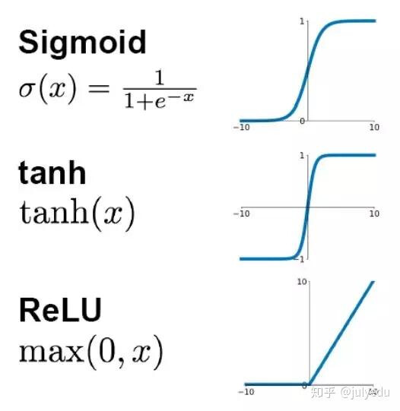
\includegraphics[width=0.28\textwidth]{../assets/figures/ch08-activations.png}}
\caption{\eng{Sigmoid}، \eng{tanh} و \eng{ReLU}. \textit{(برگرفته از تختهٔ کلاس)}}
\end{figure}

\subsection{تابع خطا، چشم‌انداز خطا و کاهش گرادیان}
خروجی با \eng{Ground Truth} مقایسه می‌شود؛ یک تابع خطا \term{میانگین مربعات خطا}{Mean Squared Error} است:
\[
\operatorname{MSE}=\frac{1}{n}\sum_{i=1}^{n}(y_i-\hat{y}_i)^2 ,
\]
که $y_i$ مقدار واقعی و $\hat y_i$ پیش‌بینی است. هدف آموزش کاهش این مقدار است.

استاد از مفهوم \term{چشم‌انداز خطا}{Loss Landscape} استفاده کرد: سطحی که ارتفاعش مقدار خطا و بقیهٔ ابعادش وزن‌هاست.

اگر مشتق خطا نسبت به وزن مثبت باشد، افزایش وزن خطا را زیاد می‌کند؛ پس باید در جهت \emph{مخالف} شیب حرکت کنیم («اگر از لاس مشتق بگیریم و مثبت شد، آن را در منفی ضرب می‌کنیم»). این مبنای \term{کاهش گرادیان}{Gradient Descent} است:
\[
\boxed{\,w_{\text{\lr{new}}}=w_{\text{\lr{old}}}-\eta\,\frac{\partial E}{\partial w}\,}
\]
که $\eta$ \term{نرخ یادگیری}{Learning Rate} (اندازهٔ گام) است: اگر بسیار کوچک باشد حرکت کند است، اگر مناسب باشد همگرا می‌شود و اگر بسیار بزرگ باشد از کمینه می‌پرد و ممکن است همگرا نشود.

\boardfigure{0.6}{ch08-learning-rate.png}{اثر نرخ یادگیری: بسیار کوچک، مناسب و بسیار بزرگ.}

\subsection{پس‌انتشار و قانون زنجیره‌ای}
سهم هر وزن در خطا با \term{قانون زنجیره‌ای}{Chain Rule} محاسبه می‌شود؛ این کار را
\term{پس‌انتشار}{Backpropagation} می‌نامند. برای نورون خروجی با
\[
\text{net}=h\,w_5+\cdots,\quad o=\sigma(\text{net}),\quad E=\tfrac12(y-o)^2 ,
\]
داریم:
\[
\frac{\partial E}{\partial w_5}=\frac{\partial E}{\partial o}\cdot\frac{\partial o}{\partial\,\text{net}}\cdot\frac{\partial\,\text{net}}{\partial w_5}
\]
\[
\boxed{\;\frac{\partial E}{\partial w_5}=(o-y)\,o\,(1-o)\,h\;}
\]
زیرا $\partial E/\partial o=o-y$ ، $\partial o/\partial\text{net}=o(1-o)$ و $\partial\text{net}/\partial w_5=h$.

\begin{figure}[htbp]
\centering
\begin{tikzpicture}[>=Stealth, font=\small]
\tikzset{unit/.style={circle,draw=mainblue,fill=softblue,minimum size=1.1cm,thick}}
\node[unit] (x) at (0,0) {$x$};
\node[unit] (h) at (3.4,0) {$h$};
\node[unit,minimum size=1.1cm,draw=gray,fill=white,dashed] (h2) at (3.4,-2.1) {$h_2$};
\node[circle,draw=mainblue,fill=softgreen,minimum size=2cm,thick] (o) at (7.2,0) {};
\draw[mainblue,thick] (o.north)--(o.south);
\node at ([xshift=-0.5cm]o.center) {\lr{net}};
\node at ([xshift=0.5cm]o.center) {\lr{out}};
\node[draw=mainblue,fill=softyellow,rounded corners=3pt,inner sep=5pt] (e) at (10.9,0) {$E=\tfrac12\,(y-o)^2$};
\draw[->,thick] (x) -- node[above] {$w_1$} (h);
\draw[->,thick,red!70!black] (h) -- node[above] {$w_5$} (o.west);
\draw[->,dashed,gray] (h2) -- node[below right,pos=0.55,inner sep=1pt] {$w_6$} (o.south west);
\draw[->,thick] (o.east) -- (e.west);
\end{tikzpicture}
\caption{شبکهٔ ساده برای پس‌انتشار و محاسبهٔ $\partial E/\partial w_5$.}
\end{figure}

\begin{correctionbox}{دقت در علامت و ضریب مشتق}
در کلاس علامت و ضریب مشتق به‌دقت تثبیت نشد. نتیجهٔ بالا برای $E=\frac12(y-o)^2$ است؛ برای تابع خطای دیگر (مثل \eng{Cross-Entropy}) جزء $\partial E/\partial o$ تغییر می‌کند و باید طبق تعریف دقیق همان تابع محاسبه شود.
\end{correctionbox}

\begin{addedbox}{مثال عددی: یک نورون، یک گام یادگیری}
ورودی $\mathbf{x}=(2,1)$، وزن‌ها $\mathbf{w}=(0.4,-0.3)$، $b=0.1$، \eng{Sigmoid} و هدف $y=1$. پیش‌رو: $z=0.6$، $o=\sigma(0.6)\approx0.646$، $E\approx0.0628$. پس‌انتشار: $\delta=(o-y)\,o\,(1-o)\approx-0.0811$ و گرادیان‌ها $\delta x_1\approx-0.162$ ، $\delta x_2\approx-0.081$ ، $\delta\approx-0.081$. با $\eta=1$: $w_1\approx0.562$ ، $w_2\approx-0.219$ ، $b\approx0.181$؛ اکنون $o\approx0.748$ و $E\approx0.0318$، یعنی خطا تقریباً نصف شد.
\end{addedbox}

چرخهٔ آموزش پنج گام دارد: مقداردهی تصادفی، \eng{Feedforward}، تولید خروجی، محاسبهٔ \eng{Loss} و \eng{Backpropagation} همراه با به‌روزرسانی وزن‌ها.

\section{مسئلهٔ هم‌نویسه در \eng{TTS}}

\term{هم‌نویسه}{Homograph} کلمه‌ای است با نوشتار یکسان و تلفظ (و معمولاً معنای) متفاوت. در فارسی چون بیشتر مصوت‌های کوتاه نوشته نمی‌شوند، این مسئله اهمیت ویژه‌ای دارد.

\begin{table}[htbp]
\centering
\caption{نمونه‌های هم‌نویسه در فارسی}
\begin{tabular}{c l l}
\toprule
کلمه & بافت اول & بافت دوم \\
\midrule
کرم & کرم مرطوب‌کننده (\eng{kerem}) & کرم خاکی (\eng{kerm}) \\
مرد & آن مرد وارد شد (\eng{mard}) & او از دنیا مرد (\eng{mord}) \\
سرم & سرم به شدت درد می‌کند (\eng{saram}) & سرم را از دستش کشیدند (\eng{serom}) \\
\bottomrule
\end{tabular}
\end{table}

\begin{correctionbox}{«شیر» هم‌نویسهٔ تلفظی نیست}
«شیر آب»، «شیر جنگل» و «شیر خوراکی» همگی \eng{/ʃir/} تلفظ می‌شوند؛ «شیر» کلمه‌ای \emph{چندمعنایی} (\eng{Homonym}) است نه هم‌نویسه با تلفظ‌های متفاوت. برای \eng{TTS} فقط مواردی مسئله‌ساز است که تلفظ‌ها فرق کنند (مانند «کرم» و «مرد»)؛ اما «شیر» مثال خوبی برای محدودیت \eng{Embedding} ثابت در فهم \emph{معناست}.
\end{correctionbox}

\textbf{نقش \eng{POS Tagging}.} گاهی \term{برچسب‌گذاری اجزای کلام}{POS Tagging} کافی است: «او مُرد» فعل و «آن مَرد» اسم است. اما «کِرم خاکی» و «کِرِم مرطوب‌کننده» هر دو اسم‌اند؛ پس به اطلاعات معنایی و بافتی، یعنی \eng{Contextual Embedding}، نیاز داریم. مثلاً «کرم خاکی» با باغچه و خاک هم‌وقوعی دارد و «کرم مرطوب‌کننده» با پوست و آرایش؛ بازنمایی کلمه باید این بافت را در خود داشته باشد.

\section{\eng{Embedding} ایستا و \eng{Word2Vec}}

\eng{Word2Vec} بر پایهٔ ارتباط هر کلمه با کلمات اطرافش آموزش می‌بیند و دو معماری دارد. بردارهای حاصل \term{ایستا}{Static} هستند: یک بردار ثابت برای هر مدخل واژگان.
\begin{itemize}
  \item \term{کیسهٔ کلمات پیوسته}{Continuous Bag of Words} (\eng{CBOW}): کلمات داخل یک \term{پنجرهٔ بافت}{Context Window} ورودی‌اند و مدل \emph{کلمهٔ مرکزی} را پیش‌بینی می‌کند (بافت $\leftarrow$ هدف)؛ بازنمایی کلمات اطراف جمع یا میانگین می‌شود.
  \item \eng{Skip-gram}: کلمهٔ مرکزی ورودی است و مدل \emph{کلمات اطراف} را پیش‌بینی می‌کند (هدف $\leftarrow$ بافت).
\end{itemize}

\begin{figure}[htbp]
\centering
\begin{tikzpicture}[rtl, >=Stealth, font=\small]
\tikzset{sq/.style={draw=mainblue,fill=softblue,minimum size=0.55cm,inner sep=0pt,thick},
 lab/.style={font=\scriptsize},
 note/.style={draw=mainblue,fill=softyellow,rounded corners=4pt,inner sep=5pt,text width=11.6cm,align=center}}
\node[note] at (5.8,4.7) {\lr{\textbf{Word2Vec}} — \lr{Static Embedding}: یک بردار ثابت برای هر کلمه\\
در زمان آموزش: \lr{Context-Based model}\\ در زمان استنتاج: \lr{Context-independent}};
% headers
\node[lab] at (0,3.1) {\lr{Input}}; \node[lab] at (2.2,3.1) {\lr{Projection}}; \node[lab] at (4.2,3.1) {\lr{Output}};
\node[lab] at (7.4,3.1) {\lr{Input}}; \node[lab] at (9.0,3.1) {\lr{Projection}}; \node[lab] at (11.0,3.1) {\lr{Output}};
% CBOW
\foreach \y/\t [count=\k] in {1.8/{W(t-2)},0.9/{W(t-1)},-0.9/{W(t+1)},-1.8/{W(t+2)}} {
  \node[sq] (c\k) at (0,\y) {}; \node[lab,left=1pt of c\k] {\lr{$\t$}}; }
\node[sq] (cp) at (2.2,0) {}; \node[lab] at (2.2,0.7) {\lr{Sum}};
\node[sq] (co) at (4.2,0) {}; \node[lab,right=1pt of co] {\lr{$W(t)$}};
\foreach \k in {1,2,3,4} \draw[->] (c\k.east) -- (cp.west);
\draw[->] (cp) -- (co);
\node[lab] at (2.2,-2.5) {(a) \lr{CBOW}};
% Skip-gram
\node[sq] (si) at (7.4,0) {}; \node[lab,left=1pt of si] {\lr{$W(t)$}};
\node[sq] (sp) at (9.0,0) {};
\draw[->] (si) -- (sp);
\foreach \y/\t [count=\k] in {1.8/{W(t-2)},0.9/{W(t-1)},-0.9/{W(t+1)},-1.8/{W(t+2)}} {
  \node[sq] (s\k) at (11.0,\y) {}; \node[lab,right=1pt of s\k] {\lr{$\t$}};
  \draw[->] (sp.east) -- (s\k.west); }
\node[lab] at (9.2,-2.5) {(b) \lr{Skip-gram}};
% goals
\node[text width=5cm,align=center,font=\footnotesize] at (1.8,-3.7) {هدف: پیش‌بینی کلمهٔ هدف \lr{(Target)} با استفاده از کلمات پیرامون \lr{(Context)}.};
\node[text width=5cm,align=center,font=\footnotesize] at (9.8,-3.7) {هدف: پیش‌بینی کلمات پیرامون \lr{(Context)} با دریافت یک کلمهٔ ورودی \lr{(Target)}.};
\node[draw=red!70!black,rounded corners=4pt,inner sep=5pt,text width=8cm,align=center,text=red!70!black,font=\footnotesize] at (5.8,-5.3) {برای کاری که کلمات نادر \mbox{\lr{(Rare words)}} زیادی دارد کدام بهتر است؟};
\end{tikzpicture}
\caption{دو معماری \eng{Word2Vec}: \eng{CBOW} و \eng{Skip-gram}، همراه با یادداشت‌های استاد روی تخته.}
\end{figure}

\begin{exambox}{پرسش استاد: برای کلمات نادر کدام بهتر است؟}
پاسخ: \eng{Skip-gram}. در \eng{CBOW} کلمهٔ نادر فقط در جایگاه «هدف» است و اطلاعات چند کلمه در یک بردار ادغام می‌شود، پس فرصت‌های یادگیری آن کم است. در \eng{Skip-gram} هر رخداد کلمهٔ نادر چند جفت آموزشی (کلمه، همسایه) می‌سازد. استاد افزود اگر داده نویز نداشته باشد حتی یک رخداد هم ممکن است اطلاعات مفیدی بدهد، اما یادگیری از نمونهٔ بسیار اندک همچنان محدود است.
\end{exambox}

\begin{correctionbox}{دقت دربارهٔ \eng{CBOW} و \eng{Word2Vec}}
در \eng{CBOW} کلمات پنجره میانگین یا جمع می‌شوند و ترتیب نقشی ندارد؛ پس همهٔ کلمات اطراف سهم برابر دارند و کلمهٔ مهم (مثلاً «مریض» برای پیش‌بینی «دکتر») وزن بیشتری نمی‌گیرد. همین انگیزهٔ مهم \eng{Attention} است. همچنین بردار مورد استفاده معمولاً از ماتریس ورودی (جدول جست‌وجو) برداشته می‌شود و در عمل برای کاهش هزینهٔ خروجی از \eng{Negative Sampling} یا \eng{Hierarchical Softmax} استفاده می‌شود. پس از آموزش فقط بردارها را نگه می‌داریم.
\end{correctionbox}

\section{محدودیت \eng{Embedding} ایستا در تشخیص هم‌نویسه}

مهم‌ترین نکتهٔ جلسه: تفاوت میان \eng{Embedding}ای که \emph{در زمان آموزش} از بافت ساخته شده و \eng{Embedding}ای که \emph{در زمان استفاده} به بافت جملهٔ جدید وابسته است.

در \eng{Word2Vec} برای «کرم» یک بردار ثابت داریم:
\[
E(\text{کرم در «کرم خاکی در باغچه بود»})=E(\text{کرم در «کرم مرطوب‌کننده را روی پوست زدم»}).
\]
این بردار در آموزش از همهٔ بافت‌ها ساخته شده (نوعی «میانگین»)، اما در استفاده برای همهٔ رخدادها یکسان است؛ پس به‌تنهایی تلفظ درست را مشخص نمی‌کند.

\textbf{راه‌حل با \eng{Embedding} ثابت:} در کنار آن یک مدل انتخاب تلفظ می‌گذاریم: \eng{Embedding} ثابت کلمه و کلمات اطراف هم‌نویسه را به مدل می‌دهیم، بخش پیش‌بینی‌کننده را با داده‌های دارای برچسب تلفظ آموزش می‌دهیم و مدل بر پایهٔ بافت تلفظ را برمی‌گزیند. اگر $z_i$ امتیاز (\eng{logit}) تلفظ $i$ام و $C$ بافت باشد:
\[
P(P_i\mid C)=\frac{e^{z_i}}{\sum_j e^{z_j}},\qquad
\hat P=\arg\max_i P(P_i\mid C).
\]
برای تعداد متفاوت تلفظ‌ها، استاد یک \eng{Linear Layer} و سپس \eng{Softmax} پیشنهاد کرد، به شرط آنکه مجموعهٔ گزینه‌ها از پیش مشخص باشد؛ معماری دقیق این بخش در جلسهٔ بعد بررسی می‌شود.

\section{چرا همهٔ تلفظ‌ها را از ابتدا برچسب نمی‌زنیم؟}
\label{sec:selfsup}

دانشجویی پیشنهاد کرد برای هر تلفظ از ابتدا یک بازنمایی جداگانه («کرم۱»، «کرم۲») داشته باشیم. استاد: از نظر مفهومی ممکن است، اما \emph{چه کسی باید تمام رخدادها را برچسب بزند؟} این کار بسیار پرهزینه است.

\begin{exambox}{تأکید استاد}
\term{برچسب‌گذاری}{Annotation} یکی از گلوگاه‌های مهم توسعهٔ سامانه‌های هوش مصنوعی است.
\end{exambox}

راه‌حل: وظایفی که برچسبشان از خود متن می‌آید، مانند \term{مدل‌سازی زبان نقاب‌دار}{Masked Language Modeling} (\eng{MLM}: پنهان‌کردن کلمات و پیش‌بینی آن‌ها) و \term{پیش‌بینی جملهٔ بعدی}{Next Sentence Prediction} (\eng{NSP} در \eng{BERT} اولیه). \eng{NSP} بیشتر یک نمونهٔ تاریخی است و پژوهش‌های بعدی (مانند \eng{RoBERTa}) نشان دادند حذفش آسیبی نمی‌زند؛ \eng{MLM} وظیفهٔ اصلی است.

\begin{definitionbox}{یادگیری نظارتی در برابر خودنظارتی}
در \term{یادگیری نظارتی}{Supervised Learning} انسان داده را برچسب می‌زند. در \term{یادگیری خودنظارتی}{Self-Supervised Learning} برچسب از خود داده ساخته می‌شود (مثلاً کلمهٔ حذف‌شده). نتیجه: نیاز به برچسب دستی کم می‌شود، استفاده از متن‌های بسیار بزرگ ممکن می‌شود و مدل بازنمایی عمومی می‌آموزد که بعداً تنظیم دقیق می‌شود. به تأکید استاد، یکی از جهش‌های بزرگ مدل‌های زبانی همین بود.
\end{definitionbox}

\section{\eng{Embedding} وابسته به بافت (پویا)}

برای اینکه \eng{Embedding} با جملهٔ ورودی تغییر کند، از \term{\eng{Embedding} وابسته به بافت}{Contextual Embedding} (پویا) استفاده می‌کنیم. در بازنمایی ایستا $E(w)=\mathbf{v}_w$ فقط به هویت کلمه بستگی دارد؛ در بازنمایی وابسته به بافت $E(w,C)=\mathbf{v}_{w,C}$ که $C$ جملهٔ حاوی کلمه است، و ممکن است $E(\text{کرم},C_1)\neq E(\text{کرم},C_2)$.

\begin{table}[htbp]
\centering
\caption{مقایسهٔ دو نوع \eng{Embedding} به روایت تختهٔ کلاس}
\begin{tabular}{p{3cm} p{5.5cm} p{5.5cm}}
\toprule
 & ایستا & وابسته به بافت \\
\midrule
تعریف & بردار خروجی تابعی از همهٔ جمله‌هایی است که کلمه در زمان آموزش در آن‌ها دیده شده & بردار خروجی تابعی از کل کلمات جملهٔ فعلی است \\
زمان استفاده & کلمه به‌تنهایی وارد جدول جست‌وجو می‌شود & کلمه در بستر جمله وارد شبکه می‌شود و بردار نهایی از رابطه با همسایه‌ها ساخته می‌شود \\
چیزی که دانلود می‌کنید & فایلی با یک سطر (مثلاً ۳۰۰ عدد) برای هر کلمه؛ «شیر» در هر معنا همان بردار است & وزن‌های شبکه (\eng{Weights \& Biases})؛ بردار کلمه تا ورود جمله وجود ندارد \\
\bottomrule
\end{tabular}
\end{table}

\section{استفاده از \eng{Attention} برای ساخت \eng{Embedding} وابسته به بافت}
\label{sec:attention}

\term{سازوکار توجه}{Attention Mechanism} سه گام دارد: (۱) نمایش همهٔ موقعیت‌های ورودی را در اختیار داشته باش؛ (۲) ارتباط هر موقعیت را با بقیه محاسبه کن؛ (۳) بر اساس وزن‌های ارتباط، اطلاعات موقعیت‌ها را ترکیب کن تا نمایش جدید هر موقعیت به‌دست آید. به‌جای ترکیب یکسان همهٔ کلمات اطراف (مانند \eng{CBOW}) مدل می‌سنجد هر کلمه چقدر مرتبط است.

\begin{itemize}
  \item \term{پرس‌وجو}{Query} ($Q$): نمایندهٔ چیزی که برایش اطلاعات می‌جوییم (کلمهٔ هدف).
  \item \term{کلید}{Key} ($K$): برای سنجش ارتباط هر کلمه با پرس‌وجو.
  \item \term{مقدار}{Value} ($V$): اطلاعاتی که بر اساس میزان ارتباط در خروجی شرکت می‌کند.
\end{itemize}
شباهت \eng{Query} و \eng{Key} (ضرب داخلی) میزان توجه به هر کلمه را می‌دهد و \eng{Value}ها با این وزن‌ها ترکیب می‌شوند. ماتریس‌های وزنی $Q$، $K$ و $V$ در آموزش یاد گرفته می‌شوند و در استنتاج ثابت‌اند؛ آنچه با جمله عوض می‌شود بردارهای محاسبه‌شده و در نتیجه خروجی است. استاد تصریح کرد \eng{Attention} فقط یک ضرب ساده نیست و هدف این جلسه درک شهودی بود. فرمول کامل:
\[
\operatorname{Attention}(Q,K,V)=\operatorname{softmax}\!\left(\frac{QK^{\top}}{\sqrt{d_k}}\right)V ,
\]
که تقسیم بر $\sqrt{d_k}$ از اشباع \eng{Softmax} در بُعد زیاد جلوگیری می‌کند.

وقتی کلمات یک توالی به کلمات همان توالی توجه می‌کنند، به آن \term{خودتوجهی}{Self-Attention} می‌گویند: اگر «کرم» کنار «خاکی» و «باغچه» بیاید بازنمایی موجود زنده ساخته می‌شود و اگر کنار «پوست» و «مرطوب‌کننده» بیاید بازنمایی دیگری. \eng{Self-Attention} هستهٔ \term{ترنسفورمر}{Transformer} است که در ادامهٔ درس می‌آید. تفاوت اصلی با \eng{Word2Vec}: شبکه در استنتاج نیز با هر جملهٔ جدید اجرا می‌شود.

\begin{correctionbox}{دقت دربارهٔ «بردار ثابت» و «بردار پویا»}
در بازنمایی وابسته به بافت وزن‌های شبکه در استنتاج عوض نمی‌شوند؛ فقط \emph{خروجی} به‌ازای جملهٔ ورودی متفاوت است. همچنین \eng{Contextual Embedding} با \eng{Transformer} یکی نیست: \eng{LSTM} دوسویه (مانند \eng{ELMo}) نیز چنین بازنمایی می‌سازد و \eng{Attention} یکی از راه‌هاست.
\end{correctionbox}

\section{پرسش و پاسخ پایان کلاس و ادامهٔ بحث}
\label{sec:qa}

استاد از دانشجویان پرسید آیا مباحث شبکهٔ عصبی باید با جزئیات بیشتر (مانند \term{مومنتوم}{Momentum}) تدریس شوند و قرار شد همین سطح مقدماتی حفظ شود. جلسهٔ بعد: بررسی دقیق‌تر لایهٔ خروجی انتخاب تلفظ و \eng{Softmax}، ادامهٔ معماری‌های مبتنی بر بافت و ورود به \eng{Transformer}.

\section{جمع‌بندی}

کلمه ابتدا با \eng{One-Hot} نمایش داده می‌شود که پراکنده است و شباهت معنایی ندارد. \eng{Embedding} متراکم و آموخته‌شده این کمبود را جبران می‌کند و \eng{Word2Vec} آن را از هم‌وقوعی کلمات می‌سازد. اما بردار \eng{Word2Vec} ایستاست و برای «کرم» در همهٔ جمله‌ها یکسان می‌ماند؛ پس برای \eng{TTS} یا مدلی روی بافت می‌گذاریم و با داده‌های برچسب‌دار آموزش می‌دهیم، یا از بازنمایی وابسته به بافت بهره می‌گیریم. چون برچسب‌گذاری دستی گران است، پیش‌آموزش خودنظارتی (مانند \eng{MLM}) اهمیت می‌یابد و \eng{Self-Attention} ابزار اصلی ساخت این بازنمایی‌هاست.

\begin{exambox}{نکات مهم برای مرور و امتحان}
\begin{itemize}
  \item تفاوت \eng{Pipeline} و \eng{End-to-End}؛ تعریف \eng{Front-End} و \eng{Back-End}.
  \item چهار محدودیت \eng{One-Hot} و مزایای \eng{Embedding} (تراکم، بُعد کم، شباهت معنایی، آموخته از داده).
  \item چرخهٔ آموزش: مقداردهی تصادفی، \eng{Feedforward}، \eng{Loss}، \eng{Backpropagation} و به‌روزرسانی؛ رابطهٔ $w_{\text{\lr{new}}}=w_{\text{\lr{old}}}-\eta\,\partial E/\partial w$ و اثر نرخ یادگیری.
  \item نقش بایاس (مثال کرایهٔ تاکسی) و تابع فعال‌سازی (غیرخطی‌کردن).
  \item \eng{CBOW} در برابر \eng{Skip-gram}؛ برای کلمات نادر \eng{Skip-gram} بهتر است.
  \item \eng{Embedding} ایستا: در آموزش وابسته به بافت، در استنتاج مستقل از بافت؛ چرا برای هم‌نویسه کافی نیست.
  \item چرا همهٔ تلفظ‌ها را برچسب نمی‌زنیم (گلوگاه \eng{Annotation}) و نقش \eng{Self-Supervised Learning}.
  \item مفاهیم \eng{Query}/\eng{Key}/\eng{Value} و فرمول \eng{Attention}.
\end{itemize}
\end{exambox}
